%%%%%%%%%%%%%%%%%%%%%%%%%%%%%%%%%%%%%%%%%%%%%%%%%%%%%%%%%%%%%%%%%%%%%%%%%%%%%%%%%%%%%%%%%
%%                                                                                     %%
%%                This file is part of the CAPH Compiler distribution                  %%
%%                            http:%/caph.univ-bpclermont.fr                           %%
%%                                                                                     %%
%%                                  Jocelyn SEROT                                      %%
%%                         Jocelyn.Serot@univ-bpclermont.fr                            %%
%%                                                                                     %%
%%         Copyright 2011-2018 Jocelyn SEROT.  All rights reserved.                    %%
%%  This file is distributed under the terms of the GNU Library General Public License %%
%%      with the special exception on linking described in file ..%LICENSE.            %%
%%                                                                                     %%
%%%%%%%%%%%%%%%%%%%%%%%%%%%%%%%%%%%%%%%%%%%%%%%%%%%%%%%%%%%%%%%%%%%%%%%%%%%%%%%%%%%%%%%%%

\chapter{Basic usage}
\label{cha:ide-basic}

We will illustrate how to write, compile and simulate with the \caph IDE with a very simple \caph
program, even simpler than that used in Part 1. This program is reproduced in
Listing~\ref{lst:ide-sample-pgm}.  It involves a single actor, named \texttt{scale}, which
multiplies by \texttt{k} each value read on its input port \texttt{i} and writes the result on its
output port \texttt{o}. This actor is instanciated once, with \texttt{k=2}, and will read inputs
from file \verb|sample.txt| and write outputs to file \verb|result.txt|.

\begin{lstlisting}[style=CaphStyle,caption={A very simple program for testing the \caph IDE},label={lst:ide-sample-pgm}]
actor scale (k: unsigned<8>)
  in (i:unsigned<8>)
  out (o:unsigned<8>)
rules i -> o
| x -> k*x
;

stream inp:unsigned<8> from "sample.txt";
stream outp:unsigned<8> to "result.txt";

net outp = scale 2 inp;
\end{lstlisting}

\medskip
First, \textbf{launch the \caph application} by clicking on its icon in the installation directory or
directly from the Windows \emph{Start} menu. 

\medskip
The application main window is shown in Fig.~\ref{fig:main-window}. 
The main elements are (with corresponding areas labeled in red in Fig.~\ref{fig:main-window}) :
\begin{enumerate}
\item a menubar
\item four buttons for file manipulation; from left to right
  \begin{itemize}
  \item create a new file,
  \item open an existing file,
  \item save a file,
  \item save all files.
  \end{itemize}
\item five buttons to invoke the compiler for
  \begin{itemize}
  \item generating the dataflow graph representation of the current program and visualize it (button \textsc{graph}),
  \item simulating the current program and visualize it (button \textsc{Simu}),
  \item generating SystemC code from the current program (button \textsc{SystemC}),
  \item generating VHDL code from the current program (button \textsc{VHDL}),
  \item generating XDF representation of the current program (button \textsc{XDF}).
  \end{itemize}
\item a tree view of the current project,
\item a tab for viewing and editing input source files,
\item a tab for viewing output files,
\item a log area, displaying issued command and outputs from the compiler.
\end{enumerate}

\begin{figure}[h]
  \centering
  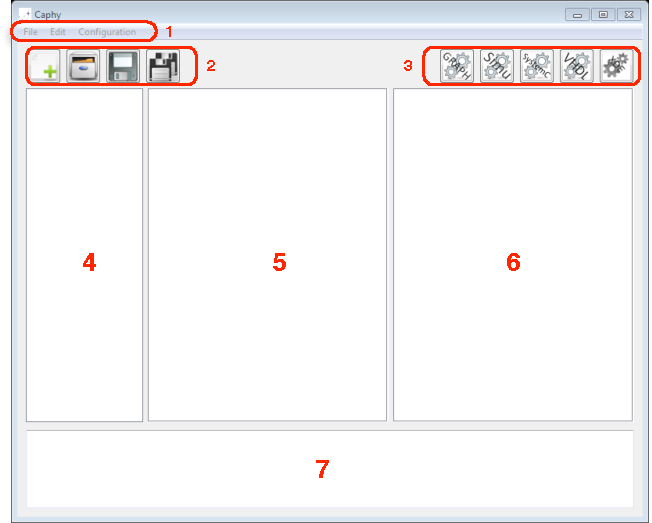
\includegraphics[width=0.75\textwidth]{figs/ide/main-window}
  \caption{\caphy main window}
  \label{fig:main-window}
\end{figure}

\medskip
Invoke the [\textsf{Configuration:Compiler and Tools}] menu item and check that the specified paths
are right (see Fig.~\ref{fig:config-window}). They should respectively point to 
\begin{itemize}
\item the location of the \texttt{caphc} compiler (\verb|<install>/bin/caphc|, where
  \verb|<install>| is the \caph installation directory, as specified during the installation
  process),
\item the location of the program to invoke for viewing \verb|.dot| graph files, 
\item the location of the program to invoke for viewing \verb|.pgm| image files. 
\end{itemize}
If the specified paths are not correct\footnote{This may be the case, for example, if you have
  changed the program to view graphs and/or images since \caph was installed.}, adjust them and click \textsc{Ok}.

\begin{figure}[h]
  \centering
  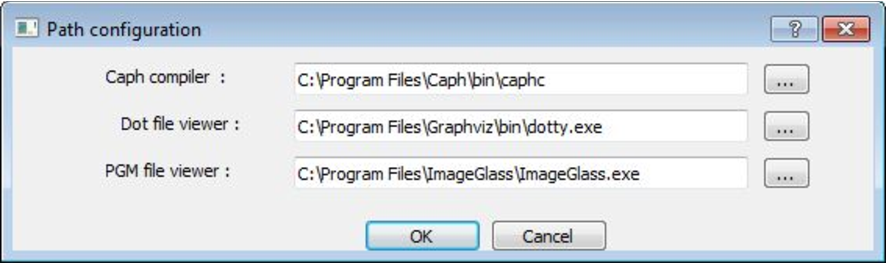
\includegraphics[width=0.75\textwidth]{figs/ide/config}
  \caption{Path configuration window}
  \label{fig:config-window}
\end{figure}

\medskip \textbf{Create a new source file} by clicking on the \textsf{New file} button (upper left)
or invoking the corresponding item of the \textsf{File} menu. A new tab will appear, named
\texttt{new} in the input files tab area. In this text tab, type\footnote{Or copy-paste} the program
reproduced in Listing~\ref{lst:ide-sample-pgm}, as illustrated in Fig.~\ref{fig:first-program}. 

\begin{figure}[h]
  \centering
  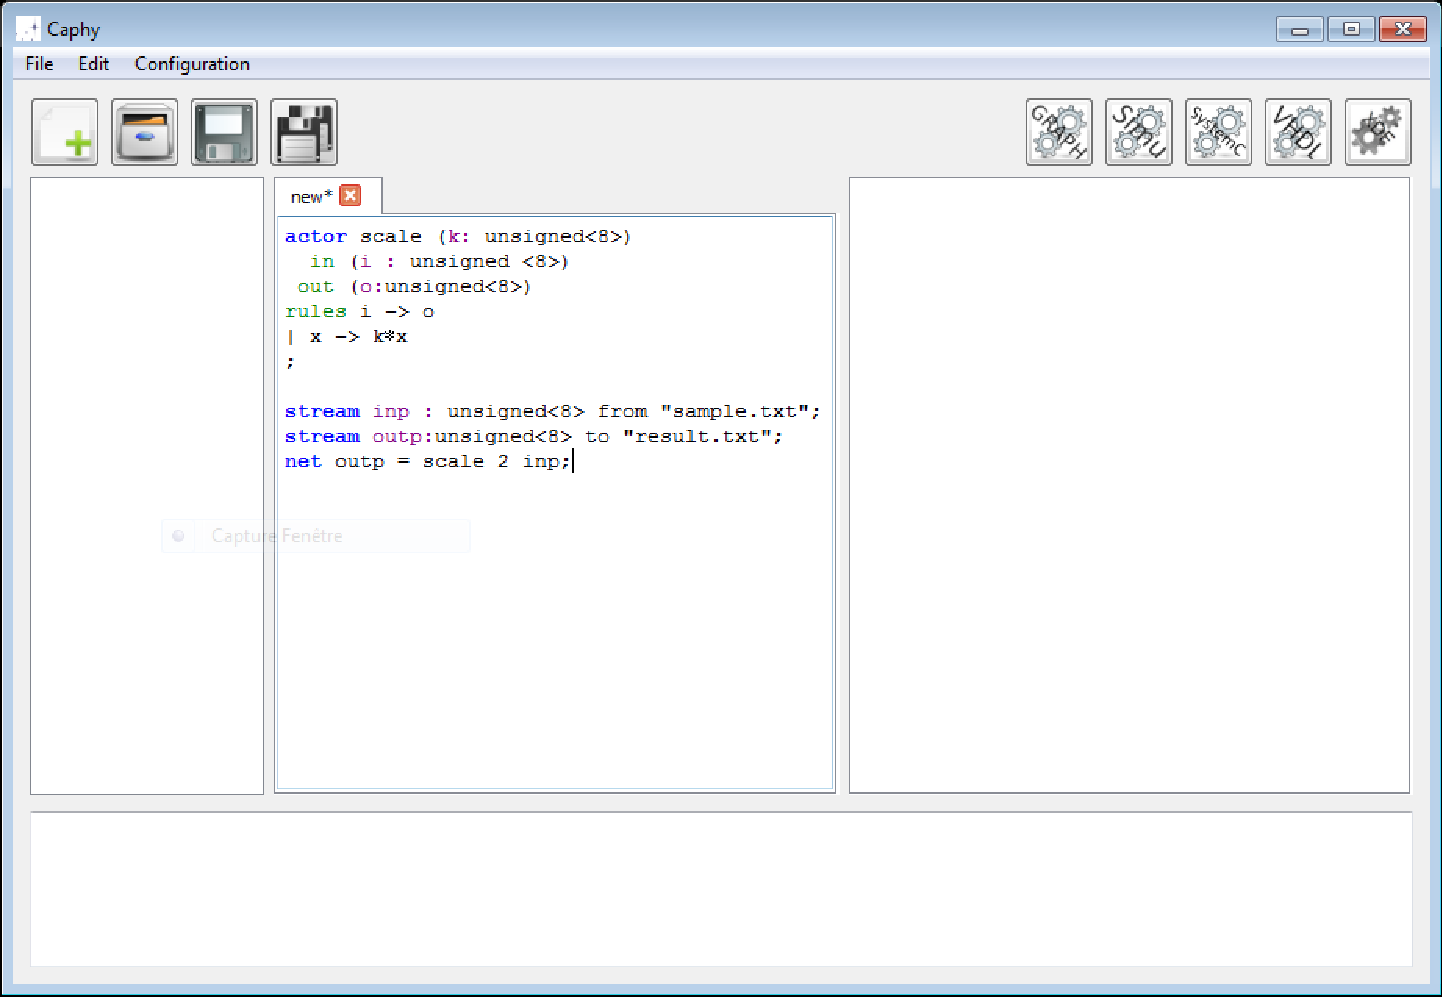
\includegraphics[width=0.75\textwidth]{figs/ide/first-program}
  \caption{Entering program}
  \label{fig:first-program}
\end{figure}

\medskip
\textbf{Save the program} by clicking on the \textsf{Save file} button or invoking the corresponding item of
the \textsf{File} menu. Be sure to use the \verb|.cph| filename suffix. Here we have saved it under
name \verb|main.cph|

\medskip
To \textbf{generate the graph}, clicking the \textsf{Graph} button (upper right). This will
\begin{itemize}
\item invoke the \caph compiler with the adequate option(s),
\item generate the \texttt{.dot} result file (in the same directory as the source file),
\item view this result by invoking the graph visualisation program specified in 
  [\textsf{Configuration : Compiler and Tools}] window.
\end{itemize}

The result is displayed in Fig.~\ref{fig:make-dot}.

\begin{figure}[h]
  \centering
  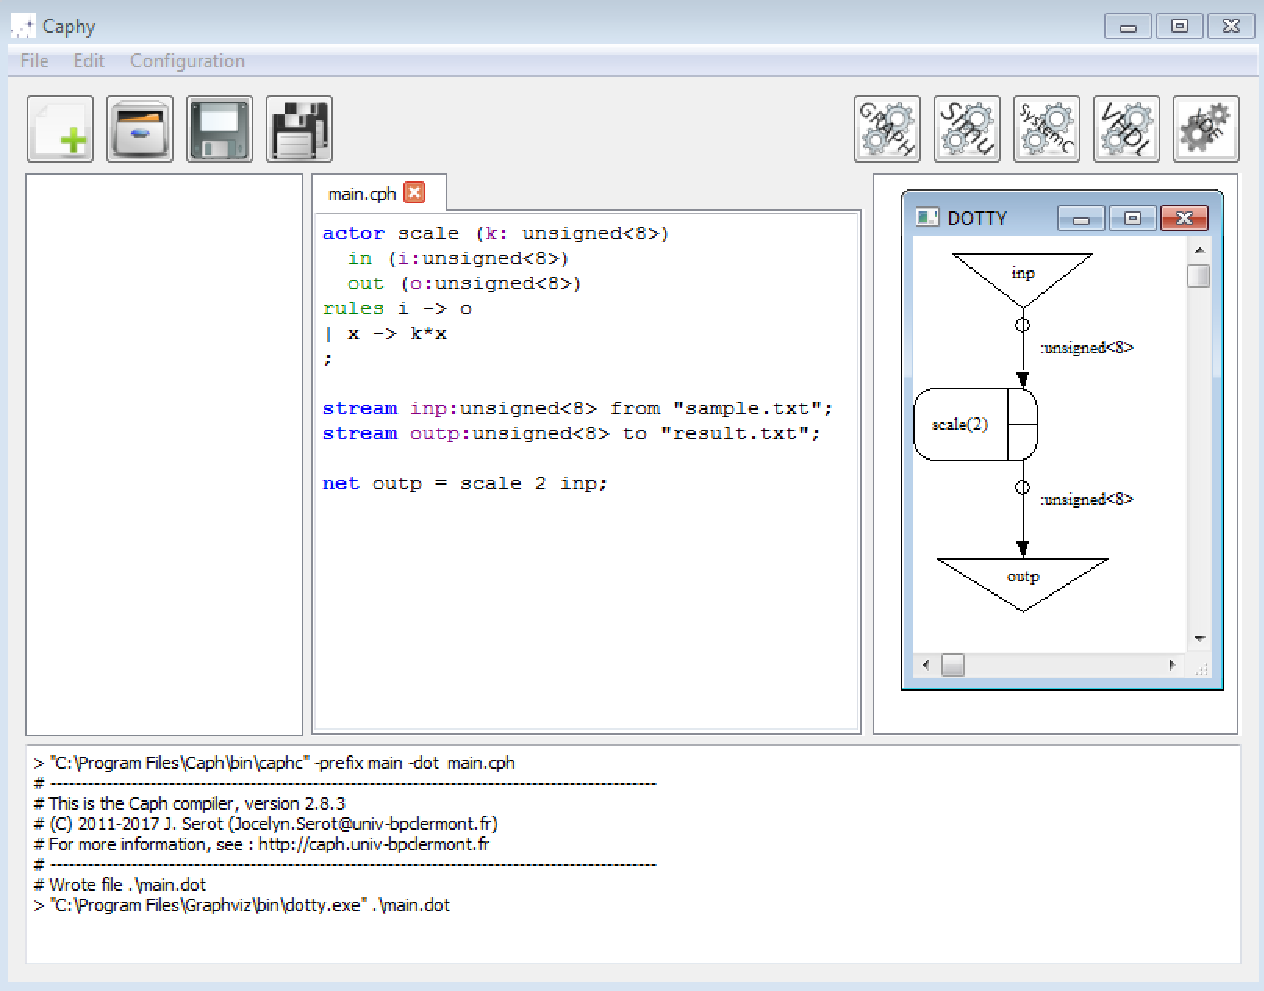
\includegraphics[width=0.75\textwidth]{figs/ide/make-dot}
  \caption{Viewing the dataflow graph of the program}
  \label{fig:make-dot}
\end{figure}

\medskip
For \textbf{simulating the program}, we first need to create the file \texttt{sample.txt} containing
the input tokens. Click on the \textsf{New File} button and type, for example, the following line in
the newly created file tab :

\begin{verbatim}
1 2 3 4
\end{verbatim}

Save the file under name \texttt{sample.txt} in the directory containing the caph source file (see
Fig.~\ref{fig:write-sample}).

\begin{figure}[h]
  \centering
  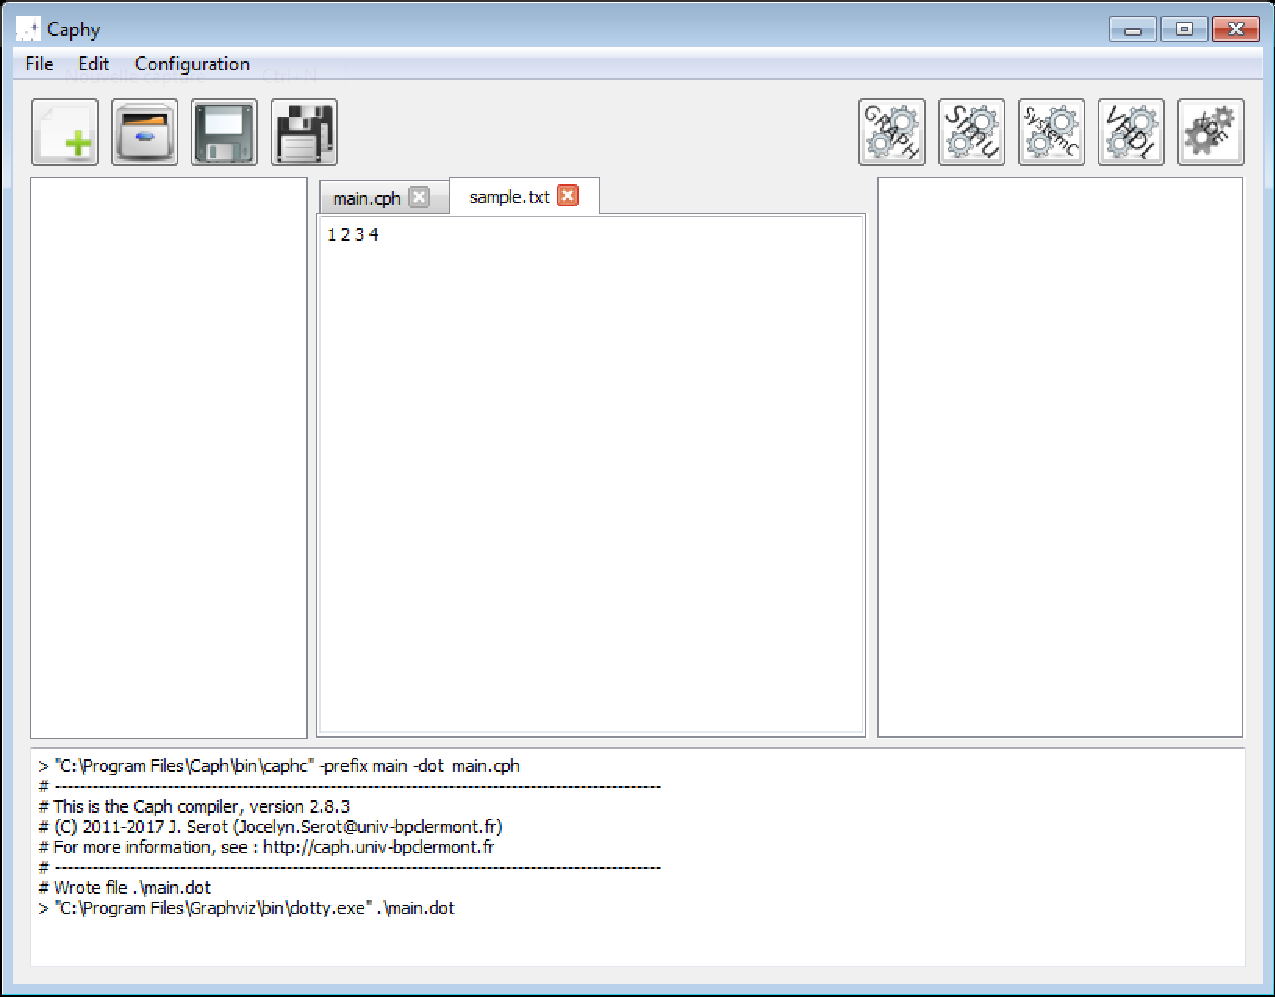
\includegraphics[width=0.75\textwidth]{figs/ide/write-sample}
  \caption{Writing the input data file for simulation}
  \label{fig:write-sample}
\end{figure}

Go back to the \caph source file by selecting the corresponding tab\footnote{Simulation will not
  work otherwise !}  and invoke the compiler by clicking on the \textsc{Simu} button. This will run
the program, generate results in the file \texttt{result.txt}\footnote{As specified by the
  \texttt{stream ... from} line in the program.} and display the latter in a separate tab, as shown
in Fig.~\ref{fig:make-sim}.

\begin{figure}[h]
  \centering
  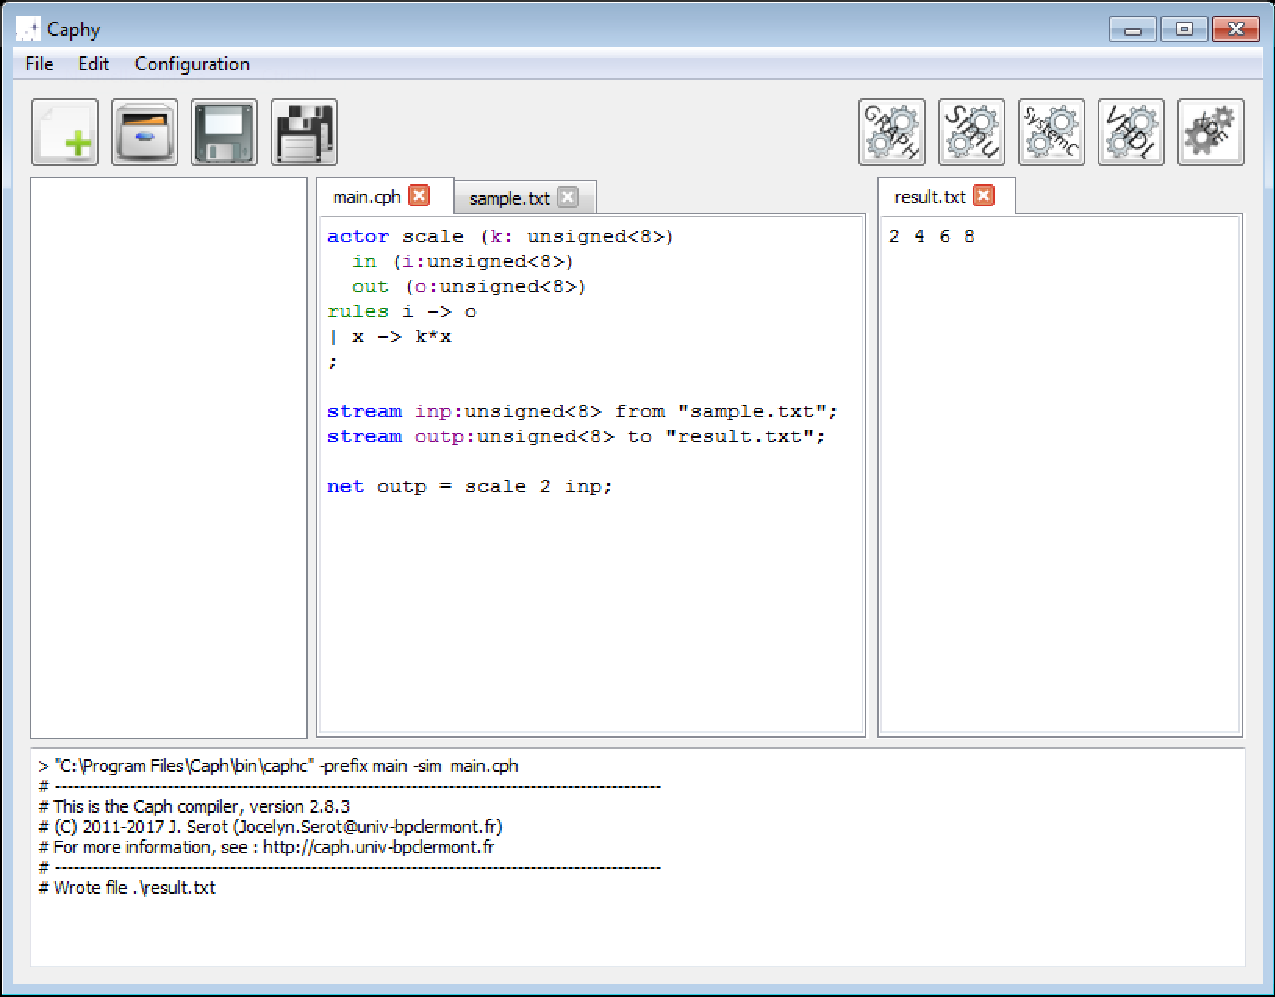
\includegraphics[width=0.75\textwidth]{figs/ide/make-sim}
  \caption{Viewing simulation results}
  \label{fig:make-sim}
\end{figure}

\medskip
For \textbf{generating the SystemC, VHDL or XDF} representation of the program, follow the procedure
described for generating the graph representation :
\begin{enumerate}
\item select the tab containing the source program
\item click on the \textsf{SystemC} (resp. \textsf{VHDL}, resp. \textsf{XDF}) button
\end{enumerate}
The result files will be generated in the same directory and displayed as separate tabs on the
right, as illustrated in figures.~\ref{fig:make-systemc} and \ref{fig:make-vhdl} respectively.

\begin{figure}[h]
  \centering
  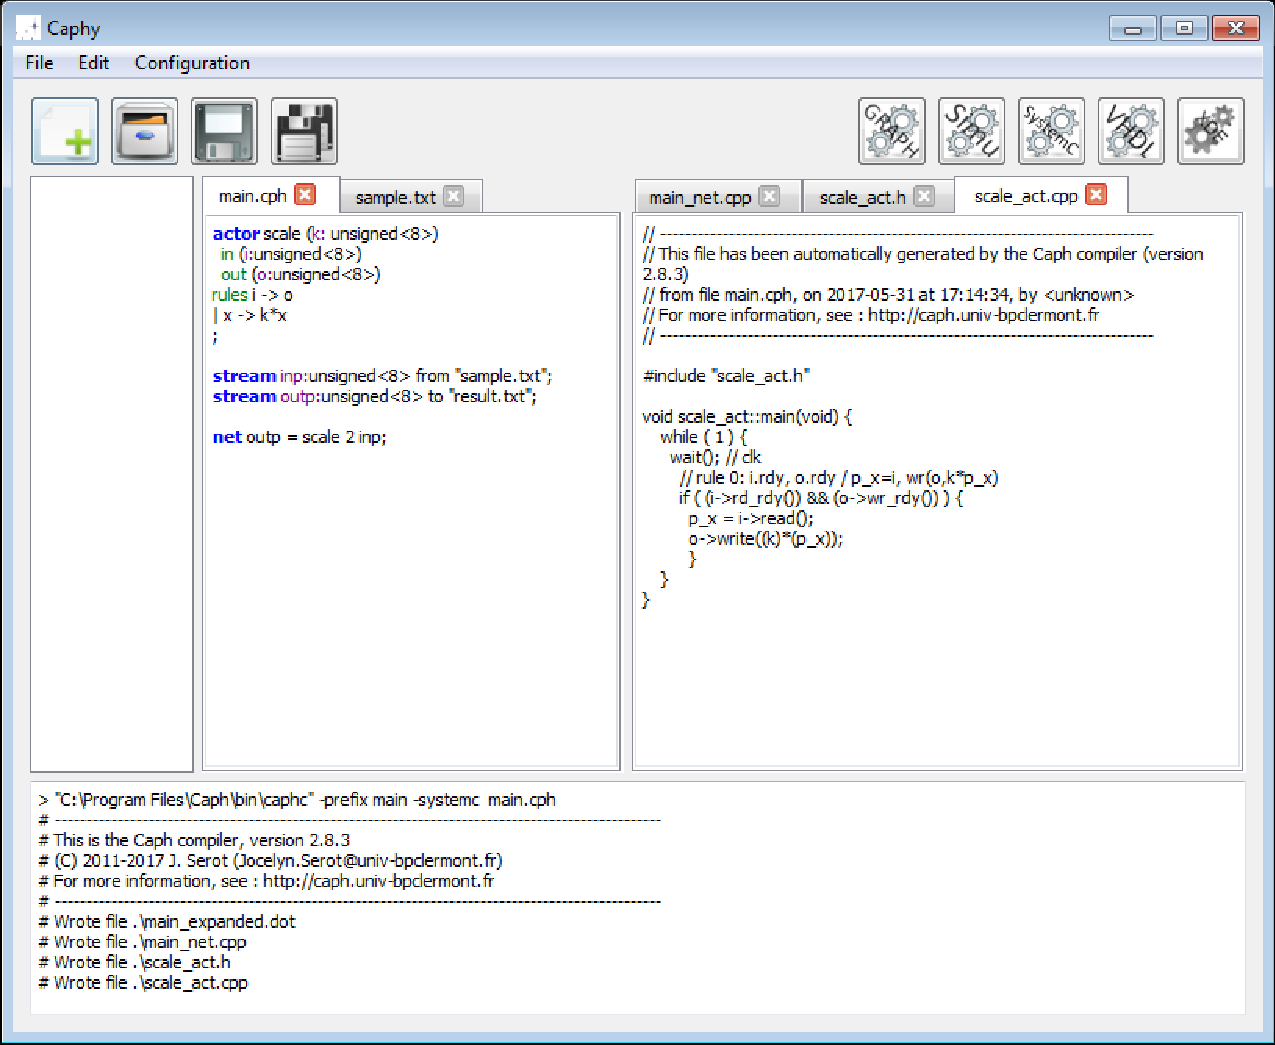
\includegraphics[width=0.75\textwidth]{figs/ide/make-systemc}
  \caption{After generating SystemC code}
  \label{fig:make-systemc}
\end{figure}

\begin{figure}[h]
  \centering
  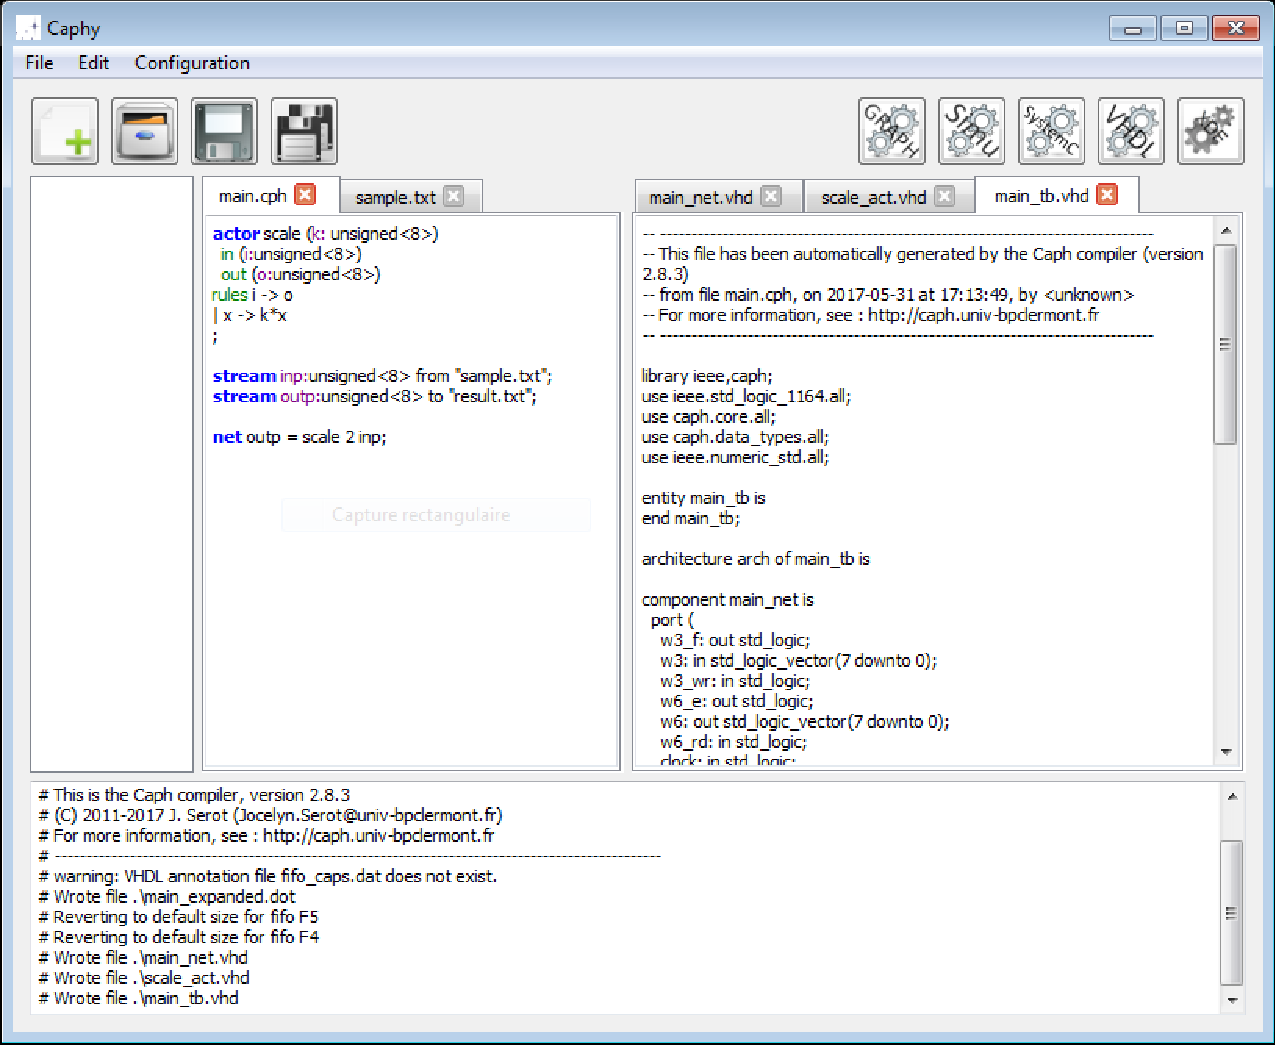
\includegraphics[width=0.75\textwidth]{figs/ide/make-vhdl}
  \caption{After generating VHDL code}
  \label{fig:make-vhdl}
\end{figure}

%%% Local Variables: 
%%% mode: latex
%%% TeX-master: "caph-primer"
%%% End: 
